
% This template has been edited from the IEEE template available at:
% https://www.ieee.org/conferences/publishing/templates.html
%
% For further help, you may wish to see:#
% https://www.overleaf.com/learn/latex/tables
% https://www.overleaf.com/learn/latex/Inserting_Images
% https://www.overleaf.com/blog/532-creating-and-managing-bibliographies-with-bibtex-on-overleaf

\documentclass[conference]{IEEEtran}
%\IEEEoverridecommandlockouts
% The preceding line is only needed to identify funding in the first footnote. If that is unneeded, please comment it out.
\usepackage[a4paper, total={6in, 8in}, margin=0.75in]{geometry}
\usepackage{cite}
\usepackage{amsmath,amssymb,amsfonts}
%\usepackage{algorithmic}
\usepackage{algorithm} 
\usepackage{algpseudocode} 
\usepackage{graphicx}
\usepackage{textcomp}
\usepackage{xcolor}
\usepackage{wrapfig}
\usepackage{subcaption}
\usepackage{comment}

\def\BibTeX{{\rm B\kern-.05em{\sc i\kern-.025em b}\kern-.08em
    T\kern-.1667em\lower.7ex\hbox{E}\kern-.125em}}

    
\begin{document}

\title{Report Title: Be Descriptive}

\author{
    \IEEEauthorblockN{Student Number}
    \and
    \IEEEauthorblockN{Student Number}
}

\maketitle

\begin{abstract}
It is normal to write the abstract last.  First, try to concisely state the problem/question/challenge under investigation.  Second, state what you found out.  The abstract should help a reader decide if they are interested in reading the whole paper.  
\end{abstract}

% 纤维约束型执行器的原理就是通过纤维约束一个方向或者一部分的弹性体形变,从而使弹性体形变时形成想要的形状。
% 本文的主题就是研究约束纤维方向对弹性体形变的影响
% 

\section{Introduction}

% 用于软机器人执行器的材料通常是各向同性的(intrinsically isotropic),即,面对外力的刺激,其各部分的应变特性是几乎相等的,这一特性使得用单一材料制成的软机器人执行器难以表现出复杂的行为。但是,如果通过引入其他材料进行约束,就可以一定程度上克服这一缺点(1)。比较适合用于进行这一约束的材料主要是各种纤维。纤维材料由于其柔韧性和柔软性(flexibility and softness),以及其作为一种常用材料的事实,使其成为一种非常适于为软机器人引入各向异性的材料。

\begin{wrapfigure}{l}{0.2\textwidth}
  \label{fig:Elastomer}
  \centering
  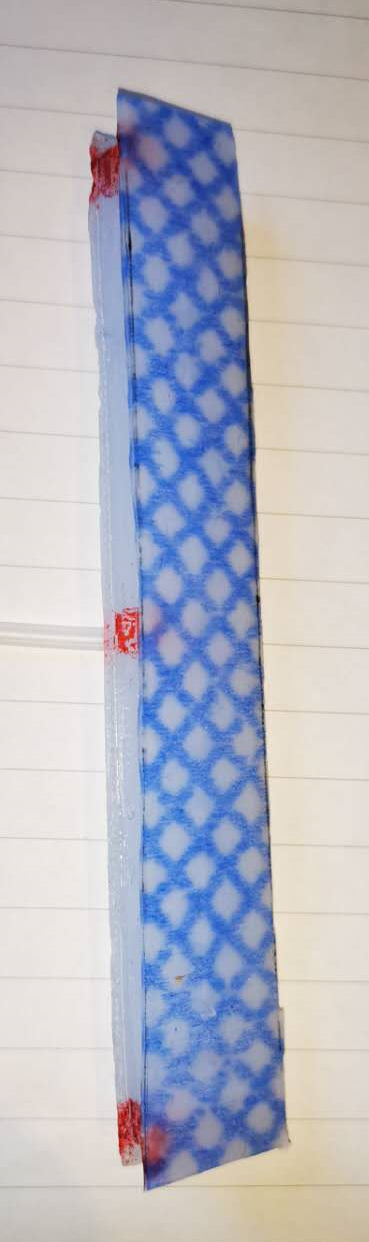
\includegraphics[width=0.15\textwidth]{pics/弹性体示意图.png}
  \caption{Elastomer gripper. The blue grid at the bottom is the strain limited layer.}
\end{wrapfigure}

The materials used for soft robot actuators are typically intrinsically isotropic, meaning that the strain characteristics of their various parts are almost equal in response to external stimuli. This property makes it difficult for a soft robot actuator made of a single material to exhibit complex behavior. However, this drawback can be partially overcome by introducing other materials as constraints. Fiber materials, due to their flexibility and softness, as well as the fact that they are a commonly used material, make them a very suitable material for introducing anisotropic properties into soft robots \cite{overview}.



% 本文中将对布里斯托大学 MSc Robotics 课程 Soft Rbotics 提供的纤维补强执行器进行研究(此处插入图片解释,全貌,受压力的形变效果)。作为一种用压力限制层(nature那个)来补强的纤维补强弹性体,其压力限制层位于长方体弹性体的一个长侧面上。有趣的是,虽然压力限制层是为了给各向同性的弹性体引入约束使其具有一定程度的各向异性特性,但是课程模组本身所提供的压力限制层(Wilco all purpose cloths)也具有各向异性,其受到水平方向拉力时产生的应变可以分解为两个正交的轴向,在一轴上较易发生轴向的应变,在另一轴上则较不容易发生轴向的应变。这就导向了一个问题:压力限制层的方向会对纤维增强弹性体的应变特性产生什么影响?
This article focuses on the fiber-reinforced gripper provided in the Soft Robotics module of the MSc Robotics program at the University of Bristol (Fig. 1). As a fiber-reinforced elastomer with a strain limited layer\cite{stress_constraint_layer}, which is placed on one of the sides of the rectangular elastomer, the interesting point is that although the strain limited layer is introduced to provide some degree of anisotropic properties to the isotropic elastomer, the stress limited layer provided in the course module  (Wilco all purpose cloths) itself is also anisotropic. When subjected to a horizontal tensile force, the cloths' strain can be decomposed into two orthogonal axial components, with axial strain being more easily generated in one axis than in the other. This leads to the question: how does the direction of the strain limited layer affect the strain characteristics of the fiber-reinforced elastomer?





\subsection{Hypothesis Statement}

% 基于以上描述,本文的假想是:使用各向异性的压力限制层来强化执行器的时候,压力限制层的方向会影响弹性体的应变特性。

Based on the description above , the hypothesis of this study is:
\begin{quote}
When using an anisotropic stress limited layer to reinforce the actuator, the direction of the stress limited layer will affect the strain characteristics of the actuator.
\end{quote}

% 此设想是受(2)启发,由于纤维补强型执行器的原理就是用纤维的应变特性来限制弹性体某一方向的形变,使其不对称从而对其进行某种物理编程(cite那个通过改变纤维角度对其进行物理编程)。对于本文中所使用的具体执行器来说,就是压力限制层会限制弹性体一侧的变形,从而使得弹性体在受到内部气压的时候向一侧弯曲,从而使其产生适合抓握的形状。如果本文的假设成立的话,此执行器就有可能通过在不同位置将压力限制层的方向对其进行进一步的物理编程,如在特定位置放置关节,使其更适合抓握。

This hypothesis is inspired by \cite{mechanical_programing}, as the principle of fiber-reinforced actuators is to use the strain characteristics of the fibers to limit the deformation of the elastomer in a certain direction, making it asymmetric and allowing for some kind of physical programming \cite{fingerlike}. For the specific actuator used in this study, the strain limited layer restricts deformation on one side of the elastomer, causing it to bend towards another side when subjected to internal pressure, resulting in a shape suitable for grasping. If the hypothesis of this study is confirmed, it may be possible to further physically program this actuator by varying the direction of the pressure-limiting layer at different positions, such as placing joints in specific locations to make the actuator more suitable for grasping.

% 本文中将会先研究压力限制层不同朝向对弹性体形变的影响,若有可见的影响,则测试此种影响用于物理编程的可能性。

This report will investigate the effect of different orientations of the strain limited layer on the deformation of the elastic body.

% 本文的结构如下:
% 1.介绍:介绍文章的研究背景与假设
% 2.设计与方法论:描述制造的过程以及实验方法论
% 3.结果与分析:描述并分析实验的结果
% 4.讨论:评价试验结果与假设的关系

The structure of this article is as follows:
\begin{enumerate}
    \item \textbf{Introduction}: Introduce the research background and hypothesis of this article.
    \item \textbf{Design and methods}: Describe the actuator manufacturing process and experimental methodology.
    \item \textbf{Results and analysis}: Describe and analyze the results of the experiment.
    \item \textbf{Discussion}: Evaluate the relationship between the experimental results and the hypothesis.
\end{enumerate}


\section{Design and methods}

\begin{comment}

\begin{algorithm}
	\caption{PPO}\label{pseudo:ppo}
	\begin{algorithmic}[1]
		\For {$iteration=1,2,\ldots$}
			\For {$actor=1,2,\ldots,N$}
				\State Run policy $\pi_{\theta_{old}}$ in environment for $T$ time steps
				\State Compute advantage estimates $\hat{A}_{1},\ldots,\hat{A}_{T}$
			\EndFor
			\State Optimize surrogate $L$ wrt. $\theta$, with $K$ epochs and minibatch size $M\leq NT$
			\State $\theta_{old}\leftarrow\theta$
		\EndFor
	\end{algorithmic} 
\end{algorithm}

It can be a good idea to include pseudocode (see Algorithm \ref{pseudo:ppo} above), and you may also want to include equations such as eq.\ref{eq:emc2} below:

\begin{equation}\label{eq:emc2}
E=mc^2
\end{equation}

\end{comment}

% 为了对比应变限制层方向对弹性体形变的影响,本文将采用如下所述的方法。


\subsection{Overview of Method}

\begin{comment}
    
Describe to the reader the general structure and procedure of your experiment. You should provide a specification a bit like a cake recipe.  For example: how long does your experiment last?  how many repeated trials do you use?  how many alternate scenarios are there?
\end{comment}

% 首先定义应变限制层的方向:相同大小的拉伸外力从不同方向作用于应变限制层时,能使应变限制层应变最大化的施力方向就是应变限制层的方向。
Firstly, the direction of the strain limited layer is defined as follows: when the same magnitude of tensile force is applied to the strain limited layer from different directions, the direction that maximizes the strain of the strain limited layer is defined as the direction of the strain limited layer.

% 为了减少实验中大量无关变量的干扰,采用的方法是:在同一抓握器的两个手指上使用不同方向的应变限制层。其中一根手指采用正常的方向(从指根指向指尖),另一根手指的应变限制层则相对正常方向有一定的倾斜。 我制作了三个抓握器,其中一个双指都为标准朝向,一个是标准+45度倾斜的组合,一个是标准+90°倾斜的组合。
To reduce the interference of a large number of irrelevant variables in the experiment, the method employed was to use strain limited layers of different directions on two fingers of the same gripper. One finger is using the standard direction (pointing from the root to the tip of the finger), while the strain limited layer on the other finger is tilted at a certain angle relative to the standard direction. I made three grippers (as shown in Fig. \ref{fig:Grippers}), one with both fingers in the standard orientation, one with a combination of standard orientation and a 45° tilt, and one with a combination of standard orientation and a 90° tilt. 

In the following text, fingers with a strain limited layer oriented in the standard direction will be referred to as the standard side, while fingers with a strain limited layer oriented in a tilted direction will be referred to as the comparing side.

% 对上图中的抓握器推入等量的空气,观察标准端和倾斜端的形变,就可以观察到应变限制层倾斜角度对弹性体应变特性的影响。具体流程如下所示:
To observe the effect of the direction of inclination of the strain limited layer on the strain characteristics of the elastomer, equal amounts of air were pushed into the grippers shown in the Fig. \ref{fig:Grippers}, and the deformation of both the standard and tilted ends were observed. The specific process is shown as follows:

\begin{algorithm}
	\caption{Experiment Process}\label{pseudo:ExperimentProcess}
	\begin{algorithmic}[1]
            \State Mark the center and both ends of the gripper in red for tracking.
            \State Place the gripper into the black square (approximately 14.4$\times$15.7cm) drawn on the paper. The specific orientation for placing the gripper is shown in Figure \ref{fig:three_images}.
            \State Use smartphone to record a video of the deformation process of the gripper as 30ml of air is slowly injected into it.
            \State Eliminate potential errors caused by screen rotation by remapping the black square corners to the corners of a 1000$\times$1000 video. 
            \State Find the coordinates of both side ends.
            \State Calculate the horizontal (y-axis of the picture) displacement of the distance between the ends of both sides from the center.
            \State When there is any displacement change on either side, record the displacement values of both sides at that time.
	\end{algorithmic} 
\end{algorithm}


\begin{figure}
    \centering
    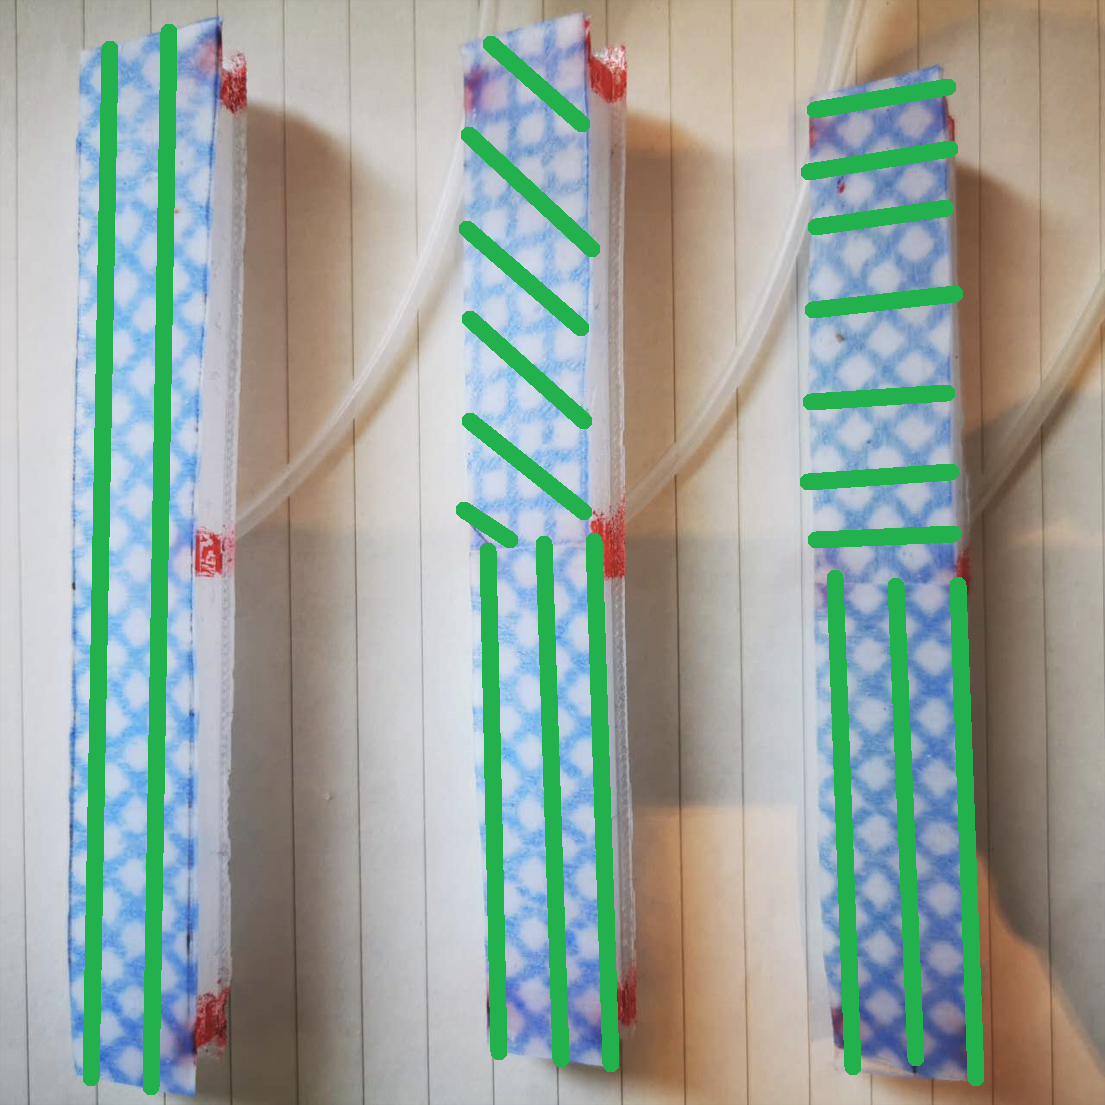
\includegraphics[width = 0.85\linewidth]{pics/实验示意图1.png}
    \caption{Grippers with different directions of strain limited layers. From left to right in the figure, they are: standard, standard $+$ 45° tilt, and standard $+$ 90° tilt. The direction of the red arrows in the figure is the same as the directions of the strain limited layer.}
    \label{fig:Grippers}
\end{figure}

\begin{figure}[htbp]
  \centering
  \begin{subfigure}[b]{0.25\linewidth}
    \centering
    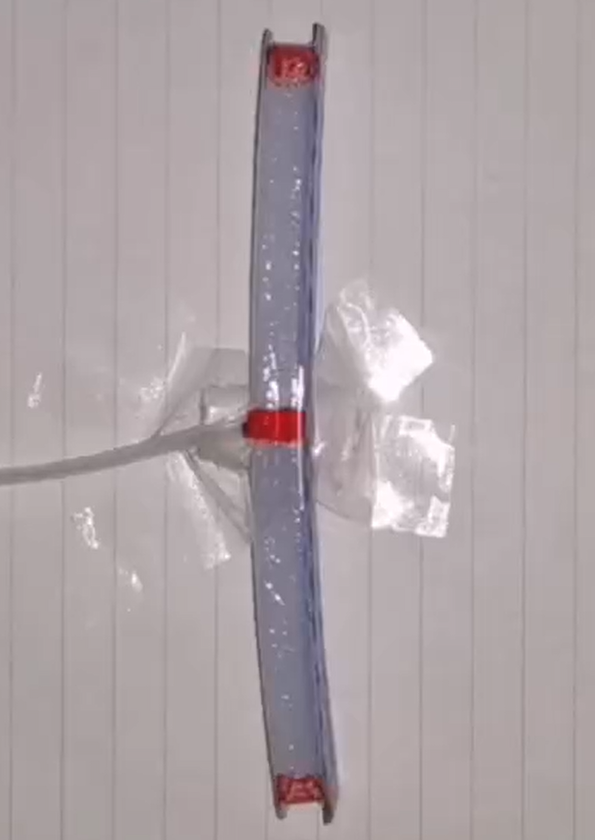
\includegraphics[width=\linewidth]{pics/变形1.png}
    \caption{}
    \label{fig:image1}
  \end{subfigure}
  \begin{subfigure}[b]{0.25\linewidth}
    \centering
    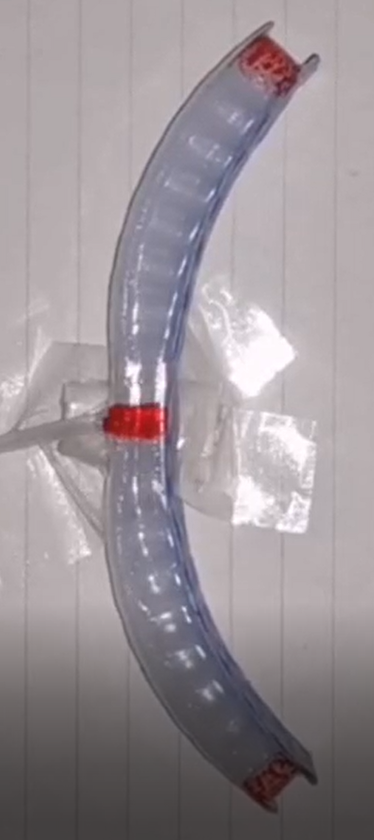
\includegraphics[width=\linewidth]{pics/变形2.png}
    \caption{}
    \label{fig:image2}
  \end{subfigure}
  \begin{subfigure}[b]{0.25\linewidth}
    \centering
    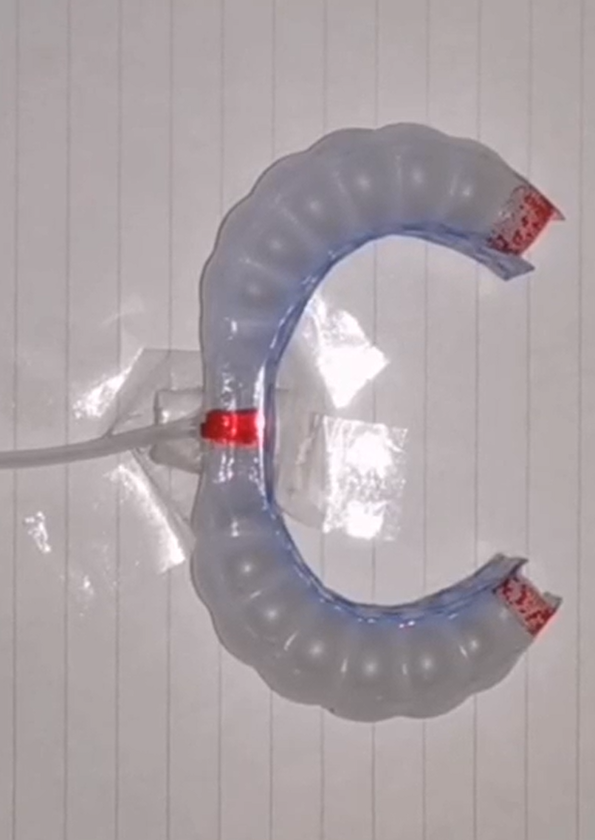
\includegraphics[width=\linewidth]{pics/变形3.png}
    \caption{}
    \label{fig:image3}
  \end{subfigure}
  \caption{Frames from the recorded video. The gripper is bending towards the positive direction of the y-axis of the picture.}
  \label{fig:three_images}
\end{figure}



\subsection{Discussion of Variables}

\begin{itemize}
    \item \textbf{Controlled Variables}: % 注入的空气多少 视频的尺寸 弹性体本身 
    \begin{itemize}
        \item \textbf{Air injected}: Use the markings on the syringe to ensure the injection of 30ml of air for each experiment.
        \item \textbf{Video size}: Always remap the black square to the size of 1000$\times$1000 pixels. This made the size of the black square irrelevant to the experiment, because I'm using the same square across the whole experiment, and it is always remapped to the same size.
        \item \textbf{Gripper}: Use the same mold to make elastomers, try to make the grippers as identical as possible. However, due to limitations in the fabrication environment, this variable is not guaranteed to be fully controlled.
        \item Direction of strain limited layer on \textbf{standard side}:  As previously shown in Fig. \ref{fig:Grippers}, the direction of the strain limited layers on the standard sides is identical.
    \end{itemize}
    \item \textbf{Independent Variable}: 
        \begin{itemize}
            \item Direction of strain limited layer on \textbf{comparing side}: As previously shown in Fig. \ref{fig:Grippers}, the direction of the strain limited layers on the comparing sides is the independent variable. 
        \end{itemize}
    \item \textbf{Dependent Variable(s)}: 
         \begin{itemize}
             \item The relationship between the horizontal displacement of the standard side end and the horizontal displacement of the comparing side.
         \end{itemize}
\end{itemize}

\subsection{Discussion of Metric(s)}

\begin{comment}
 In this section you should discuss the rationale (why) you have selected your metric(s) - e.g. how do these metrics help us to interpret your results?  Your metric(s) will need to be applied consistently throughout your experiment for them to provide a comparison of performance.  
 
 You should discuss the advantages and disadvantages of your metric(s).  Often, we need more than one metric to compensate for the information which is confused or hidden in another metric.  By using more than one metric, we can get closer to the truth of the outcome of your experiment.  
\end{comment}

% 如前所述,本实验最后会对每一个标准侧形变值获得一个对应的同等充气程度(同等压力)下的对比侧形变值。
As previously mentioned, this experiment will obtain a corresponding displacement value of the comparing side at an equivalent inflation level (which means the inner pressure is equivalent) for each displacement value of the standard side.

% 只要对于每一个标准侧位移值比较其对应的几个不同的对比侧位移值的大小,就可以简单地看出不同对比侧应变特性的区别。
 Simply by comparing  several different corresponding displacement values of the comparing side for each standard side displacement value, the differences in strain characteristics of different comparing sides can be easily observed.

 % 此metrics的好处在于,可以直观地观察出对比侧的“硬度”,
 % 不同抓握器之间的区别不会对结果有较大影响,因为对比是对比同一个标准侧位移值对应的多个对比侧位移值,实际上是用内部压力的作用结果来进行比较。由于抓握器的制作比较简单,无法保证抓握器之间的一致性,如有些抓握器腔壁比较厚,其应变特性就会改变,这时用内部压力作为指标的一部分就会不公平。
 % 此metrics的坏处在于,不能排除同一抓握器两根手指之间的区别造成的干扰。
 \textbf{Advantages}:
 \begin{itemize}
     \item The 'hardness' of different comparing sides could be easily observed.
     \item The differences between different grippers will not have a significant impact on the results. This metric concerns displacement only, and its fair to all grippers.
 \end{itemize}
 
 \textbf{Disadvantages}:
  \begin{itemize}
     \item Cannot exclude the interference caused by differences between the two fingers of the same gripper. If one finger is more "soft" than another, the experiment result will be significantly affected.
 \end{itemize}

\section{Results}

In this section you should present your results.  In general, it is best to aim for both \emph{quantitative} results (e.g., data) and \emph{qualitative} results (e.g., a written observation or graphic which is representative).  

You should use subsections where they aid in clarity.  For instance, it may be useful to present results for a ``baseline" system, then a results for an ``improved" system, and then finally results which consider both ``baseline" and ``improved" systems together.  However, this will depend entirely on your project and how you have designed your experiment.

When presenting results, aim for a presentation which clearly communicates an insight. For example, a large table of all the individual data requires the reader to do a lot of work to find out what is important.  In contrast, a table which appropriately presents the mean and standard deviation has summarised the results for the reader (and would be more useful).  Similarly, aim to combine data onto a chart when possible so that a direct comparison can be made - and when possible, include error bars.  



Remember to label all axis, caption all graphs, figures and tables, and to reference these elements in the report text (e.g. see figure \ref{fig1}) - never require a reader to have to come to their own conclusion or understanding, explain what they are looking at.  Remember to attempt to give an explanation for any anomalies in your results.  


\section{Discussion and Conclusion}

Begin your discussion and conclusion by re-stating your hypothesis.  You can literally copy-and-paste your hypothesis here.  

Because the VL1680X has been identified as an active sensor with ... limitations, we hypothesised that:
\begin{quote}
    by applying ... filtering to the sensor, we predict a measurable improvement of the sensor under ... conditions.  
\end{quote}

Make a discussion of what your results showed - whether this supported or refuted your hypothesis.  It may be that the results were mixed (supporting and refuting) and you should discuss that here. In your discussion, use this as another opportunity to demonstrate/evidence your understanding. Try to avoid stating the obvious - instead, use analysis/evaluation/synthesis to show that you understand \emph{how} and \emph{why} you saw the results you did.  What are the implications of your findings?  

This is also a good opportunity to evaluate your experiment and project as a whole.  You may wish to further discuss the limitations of the study (e.g. the difficulty of controlled/dependent variables, or any problems you faced in your project).  You may wish to make a recommendation for future work - but ensure that this is a clear advancement from the understanding you have gained and not wild speculation.


\bibliographystyle{ieeetr} 
\bibliography{ref}


\end{document}
